% STAN — compact slide version: 6 cards, no formulas, no parameter tables.
% Build: xelatex stan_architecture_slide.tex && pdftocairo -svg / -png
\documentclass[border={18pt 14pt 14pt 14pt}, multi, tikz]{standalone}
\usepackage{amsmath}
\usepackage{xcolor}
\usepackage{fontspec}
\IfFontExistsTF{Times New Roman}{
  \setmainfont{Times New Roman}
}{
  \IfFontExistsTF{Tinos}{
    \setmainfont{Tinos}
  }{
    \setmainfont{Liberation Serif}
  }
}
% math font matched to the serif text (Times -> TeX Gyre Termes Math)
\usepackage{unicode-math}
\setmathfont{TeX Gyre Termes Math}
\usetikzlibrary{positioning, fit, backgrounds, calc, arrows.meta, shadows, shapes.geometric}

\definecolor{c_in}{HTML}{4F46E5}
\definecolor{c_in_bg}{HTML}{EEF2FF}
\definecolor{c_lin}{HTML}{0284C7}
\definecolor{c_lin_bg}{HTML}{E0F2FE}
\definecolor{c_mod}{HTML}{7C3AED}
\definecolor{c_mod_bg}{HTML}{F3E8FF}
\definecolor{c_tmp}{HTML}{D97706}
\definecolor{c_tmp_bg}{HTML}{FEF3C7}
\definecolor{c_out}{HTML}{059669}
\definecolor{c_out_bg}{HTML}{D1FAE5}
\definecolor{c_arrow}{HTML}{1E293B}
\definecolor{c_muted}{HTML}{64748B}

\begin{document}
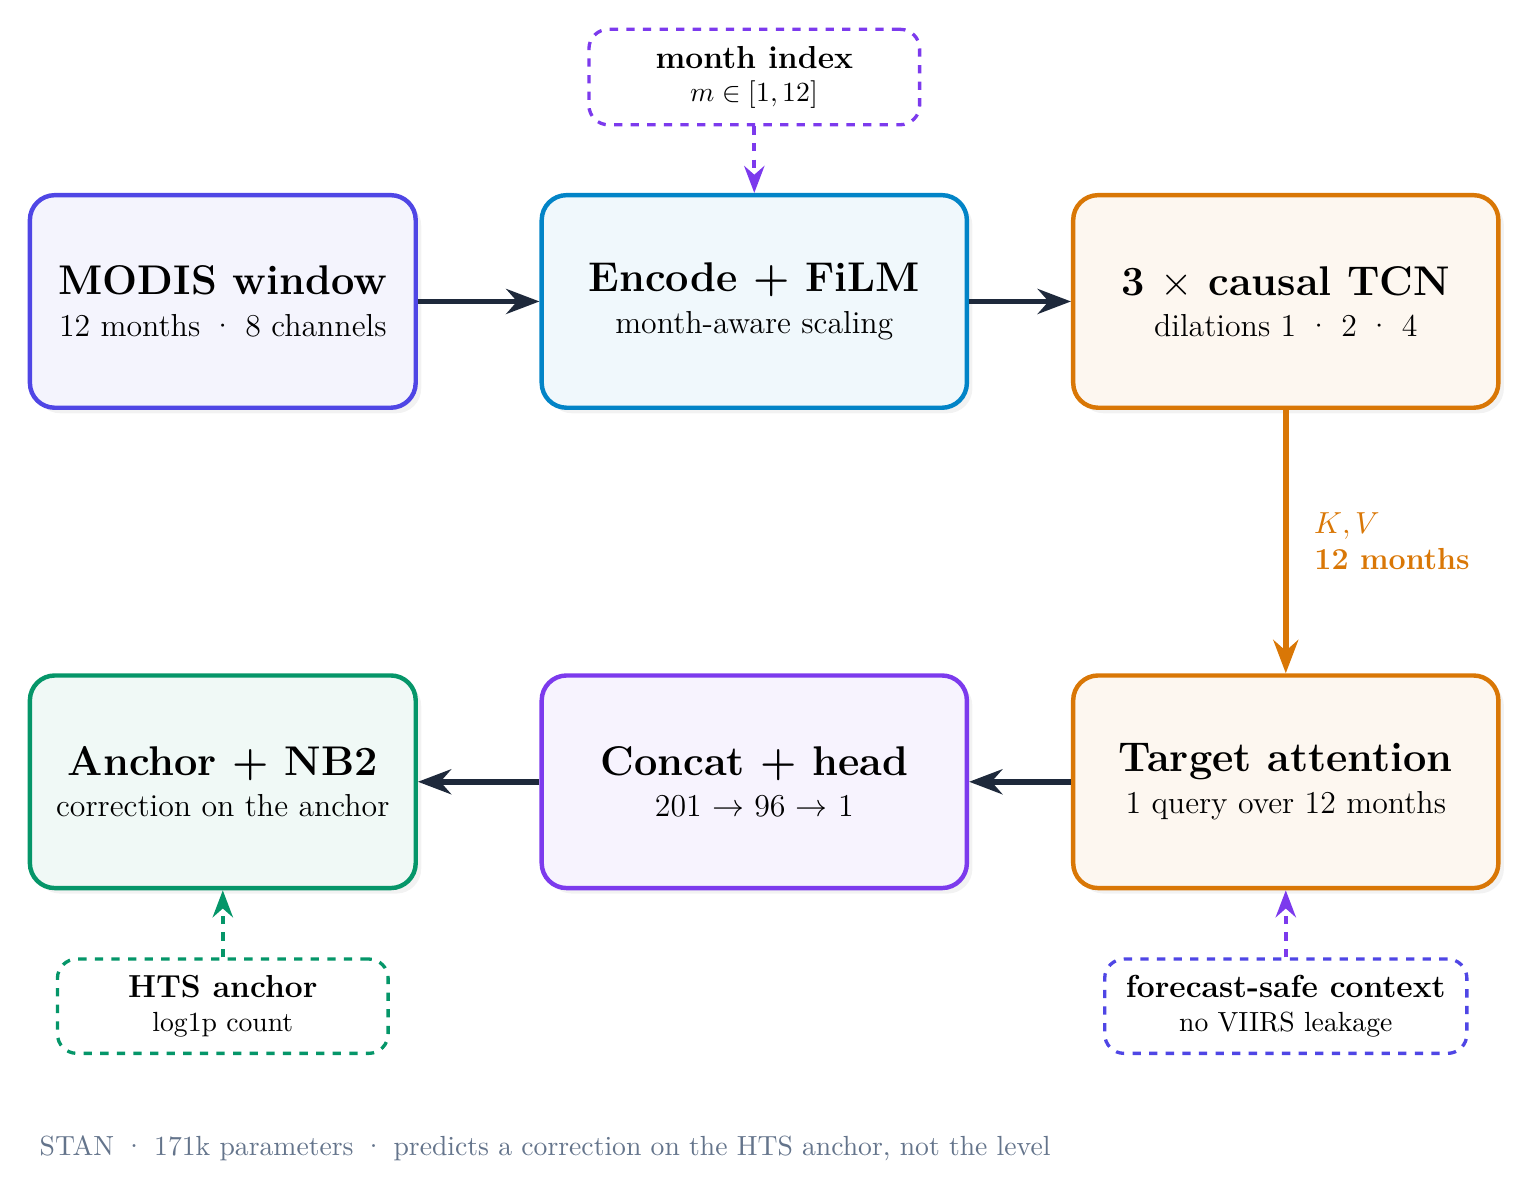
\begin{tikzpicture}[
    >=Stealth,
    card/.style={
        rectangle, rounded corners=9pt, draw=#1, line width=1.6pt,
        fill=#1!6, drop shadow={opacity=0.10, shadow xshift=2pt, shadow yshift=-2pt},
        align=center, inner sep=8pt
    },
    badge/.style={
        rectangle, rounded corners=7pt, draw=#1, line width=1.2pt, dashed,
        fill=white, align=center, inner sep=6pt
    },
    conn/.style={line width=2.0pt, draw=c_arrow, ->},
    cond/.style={line width=1.5pt, draw=c_mod, dashed, ->}
]

% ---------------------------------------------------------------- row 1
\node[card=c_in, minimum width=4.9cm, minimum height=2.7cm] (inp) at (0,0) {
    \textbf{\fontsize{15pt}{17pt}\selectfont MODIS window}\\[3pt]
    \fontsize{11.5pt}{13.5pt}\selectfont 12 months · 8 channels
};

\node[card=c_lin, minimum width=5.4cm, minimum height=2.7cm] (enc) at (6.75,0) {
    \textbf{\fontsize{15pt}{17pt}\selectfont Encode + FiLM}\\[3pt]
    \fontsize{11.5pt}{13.5pt}\selectfont month-aware scaling
};

\node[card=c_tmp, minimum width=5.4cm, minimum height=2.7cm] (tcn) at (13.5,0) {
    \textbf{\fontsize{15pt}{17pt}\selectfont 3 $\times$ causal TCN}\\[3pt]
    \fontsize{11.5pt}{13.5pt}\selectfont dilations 1 · 2 · 4
};

% month badge above the encoder
\node[badge=c_mod, minimum width=4.2cm] (month) at (6.75,2.85) {
    \textbf{\fontsize{11.5pt}{13.5pt}\selectfont month index}\\
    \fontsize{10pt}{12pt}\selectfont $m \in [1,12]$
};
\draw[cond] (month.south) -- (enc.north);

% ---------------------------------------------------------------- row 2
\node[card=c_tmp, minimum width=5.4cm, minimum height=2.7cm] (att) at (13.5,-6.1) {
    \textbf{\fontsize{15pt}{17pt}\selectfont Target attention}\\[3pt]
    \fontsize{11.5pt}{13.5pt}\selectfont 1 query over 12 months
};

\node[card=c_mod, minimum width=5.4cm, minimum height=2.7cm] (cat) at (6.75,-6.1) {
    \textbf{\fontsize{15pt}{17pt}\selectfont Concat + head}\\[3pt]
    \fontsize{11.5pt}{13.5pt}\selectfont 201 $\to$ 96 $\to$ 1
};

\node[card=c_out, minimum width=4.9cm, minimum height=2.7cm] (out) at (0,-6.1) {
    \textbf{\fontsize{15pt}{17pt}\selectfont Anchor + NB2}\\[3pt]
    \fontsize{11.5pt}{13.5pt}\selectfont correction on the anchor
};

% context + anchor badges
\node[badge=c_in, minimum width=4.6cm] (ctx) at (13.5,-8.95) {
    \textbf{\fontsize{11.5pt}{13.5pt}\selectfont forecast-safe context}\\
    \fontsize{10pt}{12pt}\selectfont no VIIRS leakage
};
\draw[cond] (ctx.north) -- (att.south);

\node[badge=c_out, minimum width=4.2cm] (anchor) at (0,-8.95) {
    \textbf{\fontsize{11.5pt}{13.5pt}\selectfont HTS anchor}\\
    \fontsize{10pt}{12pt}\selectfont log1p count
};
\draw[cond, draw=c_out] (anchor.north) -- (out.south);

% ---------------------------------------------------------------- flow
\draw[conn] (inp.east) -- (enc.west);
\draw[conn] (enc.east) -- (tcn.west);

\draw[conn, draw=c_tmp] (tcn.south) -- node[right=6pt, font=\fontsize{11pt}{13pt}\selectfont\bfseries, text=c_tmp, align=left] {$K, V$\\12 months} (att.north);

\draw[conn] (att.west) -- (cat.east);
\draw[conn] (cat.west) -- (out.east);

% ---------------------------------------------------------------- caption
\node[anchor=west, font=\fontsize{10pt}{12pt}\selectfont, text=c_muted]
    at (-2.45,-10.75) {STAN · 171k parameters · predicts a correction on the HTS anchor, not the level};

\end{tikzpicture}
\end{document}
